
\documentclass[11pt]{article}
\usepackage[utf8]{inputenc}
\usepackage{amsmath, amssymb, amsthm, csc, mathbbol}
\usepackage{float}
\usepackage{amsfonts}
\usepackage{mathtools}
\usepackage{listings}
\usepackage{multicol}
\usepackage{enumerate}
\usepackage{titlesec}
\usepackage{tikz}
\usetikzlibrary{arrows.meta,positioning}

\usepackage{graphicx}
\usepackage{fullpage}
\usepackage{comment}
\usepackage{color}
\usepackage[mathscr]{euscript}
\let\euscr\mathscr \let\mathscr\relax
\usepackage[scr]{rsfso}
\newcommand{\powerset}{\raisebox{.15\baselineskip}{\Large\ensuremath{\wp}}}
\newcommand{\myiff}{\mbox{ iff }}

\usepackage[a4paper, margin=1in]{geometry}
\newtheorem{ques}{Question}[section]
\newtheorem{defs}{Definition}[section]
\newenvironment{question}{
    \begin{ques} \normalfont
    }{
    \end{ques}
}

\newenvironment{shiftpar}[1][1.5em]
  {\list{}{%\listparindent #1%
    \itemindent\parindent
    \leftmargin#1
%    \rightmargin\leftmargin
    \parsep\z@\@plus\p@}%
    \item\relax}
  {\endlist}
  
\newenvironment{my_enumerate}{
\begin{enumerate}
  \setlength{\itemsep}{-1pt}
  \setlength{\parskip}{0pt}
  \setlength{\parsep}{0pt}}{\end{enumerate}
}

\newtheorem{claimS}{Claim}[subsection]
\newtheorem{claims}{Claim}[claimS]



\newcommand{\fdent}{\hspace{4mm}}
\titleformat*{\subsection}{\normalfont}
\newcommand{\AAND}{\; AND\;}
\newcommand{\OOR}{\; OR\;}

\newcommand*{\myfontforfunc}{\fontfamily{bch}\selectfont}
\DeclareTextFontCommand{\textfunc}{\myfontforfunc}

\lstset
{ %Formatting for code in appendix
    basicstyle=\footnotesize,
    numbers=left,
    stepnumber=1,
    showstringspaces=false,
    tabsize=1,
    breaklines=true,
    breakatwhitespace=false,
}
\renewcommand{\thesubsection}{\thesection.\alph{subsection}}


\title{CSC373 Assignment 5}
\author{Haoda Li, Ruiqi Wang}

\begin{document}
\maketitle
\begin{enumerate}
    \item To prove k-Colour is NP-complete
    \begin{enumerate}
        \item k-Colour $\in$ NP:\\
            Given undirected graph $G=(V,E)$ and $c$, where $c$ is an assignment of colors $\{1,...,k\}$ to the vertices in $G$.\\
        
            \begin{lstlisting}
    Verifier(G, c):
    for each edge e=(u, v) in E:
        if u.color = v.color:
            return false
    return true
            \end{lstlisting}
    
        \textbf{Correctness: }\\
        If $G \in$ k-Color, then there is some assignment $c$ of k colors to the vertices of $G$, s.t. no edge in G has both endpoints with same color, then the Verifier will return true for this $c$.\\
        If $G \notin$ k-Color, then for all assignments of k colors to the vertices of $G$, there is some edge in $G$ s.t. both endpoints have the same color, then the Verifier will return false for all $c$.\\[2ex] 
        \textbf{Runtime: }\\
        Looping over all the edges and checking the color of both endpoints of each edge takes $\mathcal{O}(|E|)$ time. Thus, the Verifier takes polynomial time.\\[2ex]
        From above, can conclude that k-Color is NP.\\
        
        
        \item k-Colour is NP-Hard:
        \begin{proof}
            Prove by showing that 3-Color $\rightarrow_p$ k-Color.\\
            Given an input graph $G = (V, E)$ for 3-Color:\\
            \begin{lstlisting}
    Reduction(G, c):
        V' = V \union {w_1, ..., w_{k-3}}
        E' = E \union {(w_i, v) : i = 1,...,k, v \in V'}
               \union {(w_i, w_j) : 1 <= i < j <= k-3}
        return G' = (V', E')
            \end{lstlisting}
            
        \textbf{Runtime: }\\
            Adding $k-3$ vertices and $(k-3)(k-4)/2$ edges to $G$ takes $\mathcal(O)(|V|^2)$ time, since $k \leq |V|$. Thus the reduction algo takes polynomial time.\\
            
        \textbf{Correctness: }\\
            Denote $W =  \{w_1. ..., w_{k-3}\}$.\\
            First show that: If $G \in$ 3-Color, then $G' \in$ k-Color.\\ Assign colors $k-2, k-1, k$ to vertices in $V' - W$. Since $G \in$ 3-Color, no edge in $E$ has both endpoints with same color.\\
            Then assign colors $1,.., k-3$ to vertices  $w_1. ..., w_{k-3}$. Since vertices in W all have different colors, no edge in $\{(w_i, w_j), 1\leq i < j \leq k-3\}$ has both endpoints with same color. Also, since vertices in V are assigned different colors from vertices in W, then no edge in $\{(v, w): v\in V, w\in W\}$ has both endpoints with same color.\\
            Thus, no edge in $E' = E \cup \{(w_i, w_j), 1\leq i < j \leq k-3\} \cup \{(v, w): v\in V, w\in W\} $ has both endpoint with same color. i.e. $G' \in$ k-Color.\\[2ex]
            
            Next show that: If $G' \in$ k-Color, then $G \in$ 3-Color.\\
            Since we include all possible edges between vertices in $W$, then if $G'\in$ k-Color, each vertex $w_i$ should have different color from other vertices in $W$. Thus, we need $k-3$ colors for vertices in W.\\
            Also, since we include all possible edges with one endpoint in $V$ and one endpoint in $W$, then the vertices in $V$ should have different colors from the the vertices in $W$. Then there is only $3$ colors left to assign to vertices in $V$. And since $G' \in$ k-Color, no edge in $E$ has both endpoints with same color. Thus, the original graph $G \in$ 3-Color.
        \end{proof}
            From above, can conclude that k-Color is both NP and NP-hard and thus NP-complete.\\[2ex]
        
    \end{enumerate}
    
    \item Define 3-COLOUR-SEARCH such that \\
    Input: an undirected graph $G=(V,E)$\\
    Output: if a coloring exists, $C=\{c_1,...,c_n\}$ where $c_i\in\{0,1,2\}$ is the colouring of $v_i$ for $i\in\{1,2,...,n\}$. If no colouring exists, return $Nil$.  \\
    In the algorithm, we will represent vertices using disjoint sets. At the beginning, each vertex is stored in one set. Then, by merging two vertices, we call union on the two vertices. 
    Then, the algorithm is:
    \begin{lstlisting}
3-COLOUR-SEARCH(G):
    if not 3-COLOUR(G):
        return Nil
    while G has more than 3 vertices:
        # we will prove such pair of vertices exists in each iteration
        find one pair of non-adjacent vertices u, v and 
        3-COLOUR(merge(G,u,v))
        # merge(G,u,v) returns G with u, v merged
        G = merge(G,u,v)
    colour each vertices set in G with one colour
    \end{lstlisting}
    \textbf{Correctness} \\
    Let $G_i$ be the graph after $i$th iteration of the for loop. $G_0$ is the graph before the for loop.\\
    \textbf{Claim}. For each $i\in\mathbb{N}$, $G_i$ is 3-colour-able.
    \begin{proof}
    This claim is trivial since line 1-2 makes sure $G_0$ is 3-colour-able and for each iteration $3-COLOUR(merge(G,u,v))$ makes sure $G$ after each iteration is also 3-colour-able.
    \end{proof}
    \textbf{Claim.} For each iteration of the while loop, we can always find one pair of non-adjacent vertices u, v and $3-COLOUR(merge(G,u,v))$.
    \begin{proof}
    Let $G_i$ be the graph after the $i$th iteration of the while loop for $i\in\mathbb{N}$, consider $G_{i+1}$, by the claim above, we know that $G_i$ is 3-colour-able and by the while condition, $G_i$ has more than 3 vertices. Therefore, there must exists a pair of vertices $u,v$ that have the same colour for a valid 3-colouring in $G_i$. They must be non-adjacent, or it violates the colouring constraint. Also, $merge(G_i,u,v)$ is 3-colour-able with the same colouring of $G_i$. Given all vertices in $merge(G,u,v)$ the same colour as in $G_i$, the merged vertex $uv$ is the colour of $u$ and $v$, since $u,v$ has the same colour. Any vertices adjacent to $u$ or $v$ still have the different colouring from the merged vertex $uv$, and any vertices not adjacent to $uv$ have the same connectivity and colouring-validity as in $G_i$. 
    \end{proof}
    \textbf{Corollary} When the while loop exits, $G$ has 3 vertices sets (exits by the while condition). \\
    Since we know the while loop will exit, Let $G_n$ be the the graph in line 10 after the while loop. \\
    \textbf{Claim.} The colouring by line 10 is a valid 3-colouring for all $G_{i}, i\in\mathbb{N}. i\leq n$.
    \begin{proof} 
    We will induce from n back to 0. \\
    Base case: Since there are only $3$ vertices in $G_n$, each has distinct colour, it must be a valid 3-colouring. \\
    Inductive steps: Consider the $i$th iteration of the while loop, assume the colouring is valid for $G_i$, consider $G_{i-1}$. Since $G_{i}$ is obtained by merging some vertices $u, v$ in $G_{i-1}$. split $u,v$ and all the edges attached with the same way as we merge $u,v$. Since $u,v$ are non-adjacent by line 6, they can still have the same colouring in $G_{i-1}$. For any vertices to $u$ or $v$, they are adjacent to $uv$, hence the colouring for them is valid in $G_{i-1}$. For any vertices not adjacent to any of $u$ or $v$, they maintain the same connectivity and colouring-validity as in $G_{i}$. Therefore, the colouring is still valid for $G_{i-1}$.\\
    By induction, the claim is proven. Therefore the colouring is valid for $G_0$, which is the input graph. And the algorithm is correct. 
    \end{proof}
    
    
    
    
    \textbf{Runtime} Let $n=|V|, m=|E|$. 
    Assuming $3-COLOUR(G)$ takes $t(n)$ time. Then, since each iteration will merge one pair of vertices, each iteration will reduce the total number of vertices by one and the while loop exits when there are 3 vertices. There are at most $n-3$ iterations of the for loop. For each iteration, there are at most $(n-i)(n-i-1)$ pairs of non-adjacent vertices, where $i$ is the number of iteration, and merging takes at most $O(m)$ time. Therefore, the total runtime of the while loop is $\sum_{i=0}^{n-3} (n-i)(n-i-1)(m+t(n))\in O(n^3(m+t(n)))$. The final colouring will take at most $n$ time. Then, the total run time is at most $O(n^3(m+t(n)))$. The time is polynomial to $t(n)$. \\[2ex]
    
    
    
    \item
    \begin{enumerate}
        \item Greedy Algorithm: 
        \begin{lstlisting}
  Result = Empty list
  B = sorted list of (i, j) in decreasing order of a_ij
  for each b = (u, v) in B:
      if((u-1,v),(u+1, v),(u, v-1),(u, v+1) all not in Result):
          add b to Result
        \end{lstlisting}
        
        \textbf{Counter Example: }\\
        let $a_{22} = 100$, $a_{12} = a_{21} = a_{32} = a_{23} = 99$, $a_{11} = a_{13} = a_{31} = a_{33} = 1$.\\
        The Greedy algorithm will choose  $(2, 2), (1, 1), (1, 3), (3, 1), (3, 3)$, with a total of 104 traffic accidents reduced.\\
        However, the optimal solution is to choose $(1, 2), (2, 1), (3, 2), (2. 3)$ with a total of 396 traffic accidents reduced.\\
        
       
        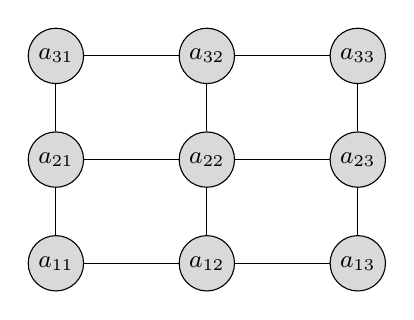
\begin{tikzpicture}[
      mycircle/.style={
         circle,
         draw=black,
         fill=gray,
         fill opacity = 0.3,
         text opacity=1,
         inner sep=0pt,
         minimum size=20pt,
         font=\small},
      myarrow/.style={-Stealth},
      node distance=0.6cm and 1.2cm
      ]
      \node[mycircle] (c1) {$a_{31}$};
      \node[mycircle,right=of c1] (c2) {$a_{32}$};
      \node[mycircle,right=of c2] (c3) {$a_{33}$};
      \node[mycircle,below=of c1] (c4) {$a_{21}$};
      \node[mycircle,right=of c4] (c5) {$a_{22}$};
      \node[mycircle,right=of c5] (c6) {$a_{23}$};
      \node[mycircle,below=of c4] (c7) {$a_{11}$};
      \node[mycircle,right=of c7] (c8) {$a_{12}$};
      \node[mycircle,right=of c8] (c9) {$a_{13}$};
      

 \foreach \i/\j in {% start node/end node/text/position
      c1/c2,
      c2/c3,
      c4/c5,
      c5/c6,
      c7/c8,
      c8/c9,
      c1/c4,
      c2/c5,
      c3/c6,
      c4/c7,
      c5/c8,
      c6/c9}
       \draw [] (\i) -- node[sloped,font=\small,\p] {} (\j);
    \end{tikzpicture}
    
    Thus, the Greedy algorithm does not always find the optimal solution.\\[2ex]
    
    \item The approximation ratio is 4.\\
    Since this is a maximization problem, we need to show that $\forall m,n \in \N^+$ and $\forall$ input $x = (a_{ij})_{m\times n}$, the result $G(x)$ of the greedy algorithm satisfies $4 \cdot G(x) \geq OPT(x)$.\\
    \begin{proof}
         Let $m, n \in \N^+$, $x = (a_{ij})_{m\times n}$ be an input of size $mn$.\\
         Let $S$ be the selection returned by the greedy algorithm and let T be any other valid selection of intersections.\\[2ex]
         Claim:  $ \forall (i, j) \in T$, either $(i, j)\in S$ or there is an adjacent $(i', j') \in S$ with $a_{i'j'} \geq a_{ij}$.\\[2ex]
         Justification for claim: \\
         Case 1: If all adjacent intersections $(i', j')$ to $(i, j)$ have $a_{i'j'} < a_{ij}$, then the Greedy algorithm will pick $(i, j)$, since none of its adjacent intersections will be picked before $(i, j)$ is picked.\\
         Case 2: If $(i, j)$ has some adjacent intersections with more or equal accidents able to be prevented.\\
         If such adjacent intersection is in S, then the proof for claim is done.\\
         If not, when the greedy algorithm making decision on $(i, j)$, none of its adjacent intersections is picked, since the intersections $(i', j')$ with $a_{i'j'} > a_{ij}$ are considered before (i, j) but not added to S, and the intersections with $a_{i'j'} < a{ij}$ has not been considered yet, while for those adjacent intersections $(i', j')$ with $a_{i'j'} = a_{ij}$, either they are considered before $(i, j)$ but not added to S, or they have not been considered yet. Then the Greedy Algorithm will pick $(i, j)$.\\[2ex]
         
         Thus, for the optimal solution $T^*$ and $(i^*, j^*) \in T^*$, either $(i^*, j^*)\in S$ or there is an adjacent $(i', j') \in S$ with $a_{i'j'} \geq a_{i^*j^*}$. Then let $b_{i^*j^*} = max\{a_{ij}: i=i^*, i^*\pm 1, j= j^*, j^* \pm 1, (i, j) \in S\}$, we have  $b_{i^*j^*} \geq a_{i'j'} \geq a_{i^*j^*}$ and \\
         $$OPT(x) = \Sigma_{(i, j) \in T^*} a_{ij} \leq \Sigma_{(i, j) \in T^*} b_{ij} (*)$$
         Since each intersection has at most four adjacent intersection in T or is itself in T, each intersection in S is summed up at most four times in (*). Thus $4 \cdot G(x) \geq OPT(x)$.\\ 
    \end{proof}
    
    \end{enumerate}  
\end{enumerate}

  


\end{document}
